\documentclass{standalone}

\usepackage{tikz}
\usetikzlibrary{arrows}
\usetikzlibrary{decorations.pathmorphing,patterns}
\usepackage[papersize={3in,2in},margin=0in]{geometry}

\begin{document}
  

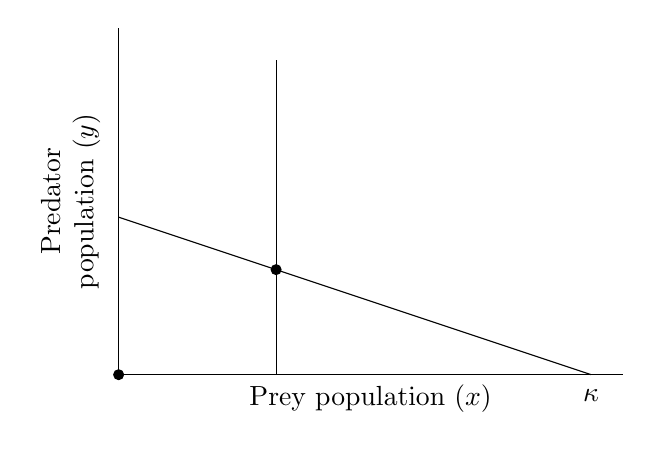
\begin{tikzpicture}[scale=2]
\draw (0,0) -- (3.2,0) node[pos=.5, below]{Prey population ($x$)};  
\draw (0,0) -- (0,2.2) node[pos=.5, sloped, above=2pt]{\begin{tabular}{c}Predator \\ population ($y$)\end{tabular}};
\draw (1,0) -- (1,2);
\draw (0,1) -- (3,0) node[below=2pt]{$\kappa$};
\fill (1,0.667) circle(1pt);
\fill (0,0) circle(1pt);
\end{tikzpicture}


\end{document}

